
%  \section{The analysis of FWHM behavior} 

Given that the observed seeing is by and large described by a single parameter, FWHM, 
we study here three aspects of its variation in detail: dependence on wavelength,
the spatial (angular) structure function, and temporal behavior. We note that details 
about the seeing profile tails, including the contribution of the instrumental profile and
the $i$ band behavior, do not matter here because we focus only on the FWHM behavior. 

\subsection{The FWHM dependence on wavelength} 

The Kolmogorov turbulence theory gives a standard formula for the FWHM of a long-exposure
seeing-limited PSF in a large telescope,
\begin{equation}
\textrm{FWHM}^{\rm Kolm}(\lambda, X) = \frac{0.976\lambda}{r_0(\lambda,X)}.
\label{eq:fwhmkolm}
\end{equation}
Here $\lambda$ is the wavelength, $X$ is the airmass, and $r_0$ is the Fried parameter.
We use $\lambda = 500$ nm as the reference wavelength,
\begin{equation}
\label{eq:airmass}
r_0(\lambda,X) = r_0(500) \left(\frac{\lambda}{500}\right)^{1.2}
\frac{1}{X^{0.6}},
\label{eq:r0}
\end{equation}
where $r_0(500)$ is the $r_0$ for $\lambda=500$ nm and $X$=1, and $\lambda$ is 
expressed in nm.
Substituting Eq.~(\ref{eq:r0}) into (\ref{eq:fwhmkolm}), it is easy to show that 
\begin{equation}
\textrm{FWHM}^{\rm Kolm} \propto \lambda^{-0.2}.
\end{equation}


With the \vk~atmosphere model, the FWHM as in
Eq.~(\ref{eq:fwhmkolm}) needs an additional correction factor
which is a function of the outer scale $L_0$~\citep{Tokovinin2002},
\begin{equation}
\label{eq:FWHMvK}
\textrm{FWHM}^{\rm vonK}(\lambda, X) = \frac{0.976\lambda}{r_0(\lambda,X)}
\sqrt{1-2.183\left( \frac{r_0(\lambda,X) }{L_0} \right)^{0.356}}.
\end{equation}
If a power-law approximation is attempted,  FWHM$^{\rm vonK} \propto \lambda^{\alpha} $, 
$\alpha$ becomes a function of $L_0$ and $r_0$ at a specified
wavelength and airmass, or equivalently, a function of $L_0$ and FWHM$^{\rm vonK}$.
For the subsequent analysis, we adopt the $r$ band as the fiducial band (with
the effective wavelength of 616.6 nm).


\begin{figure}[th]
\centering
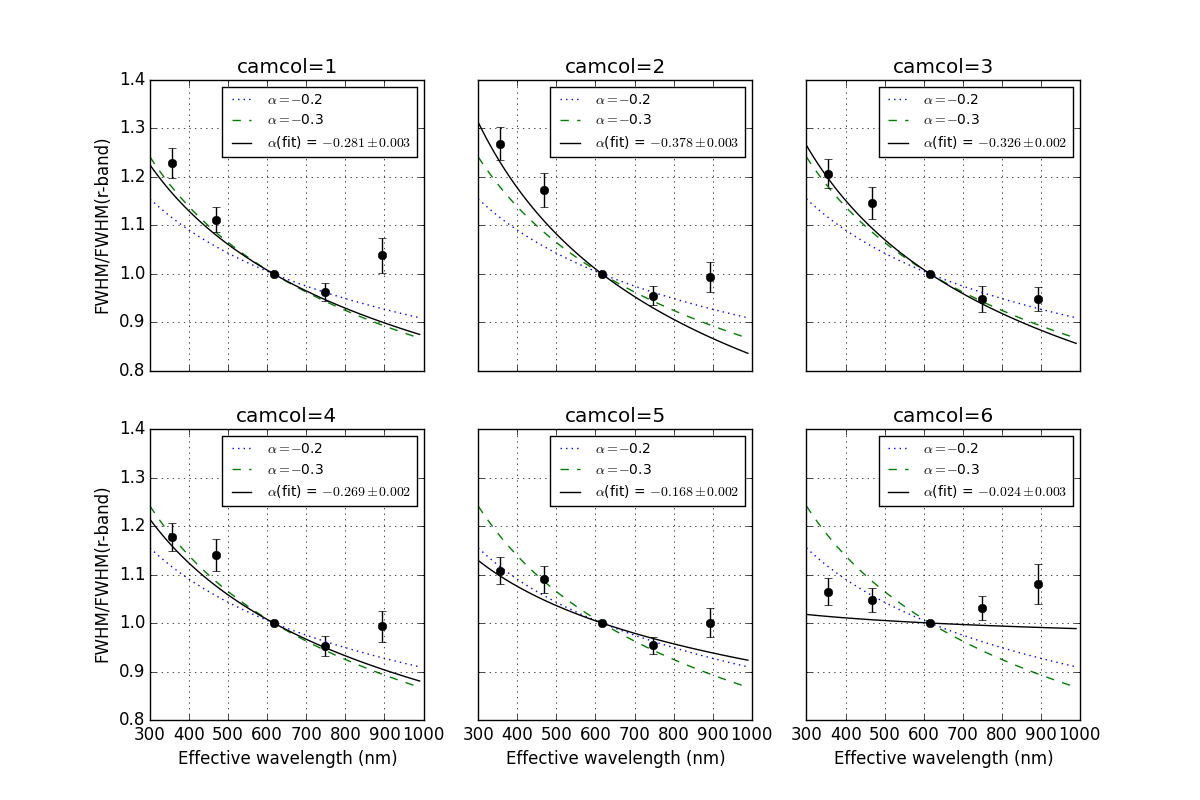
\includegraphics[width=0.9\textwidth]{FIGURES/fwhm_lambda.png}
\caption{The behavior of FWHM as a function of wavelength for the fiducial run 4874.
Symbols are SDSS data and solid line is the best power-law fit, with the best-fit slope
($\alpha$) shown in inset. For comparison purposes, the $\alpha=-0.2$ (dotted) and $\alpha=-0.3$ 
(dashed) lines are also shown. For the ensemble behavior of best-fit $\alpha$, see Fig.~\ref{fig:alpha_fwhm}. 
\label{fig:fwhm_lambda}}
\end{figure}


\begin{figure}[th]
\centering
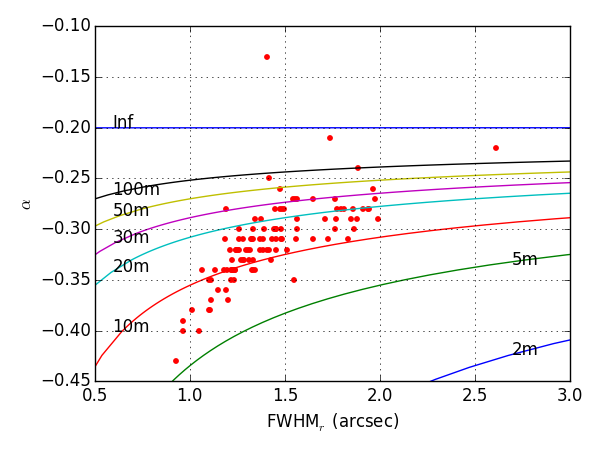
\includegraphics[width=0.8\textwidth]{FIGURES/alpha_fwhm.png}
\caption{The variation of the best-fit power-law index for the wavelength dependence of FWHM, $\alpha$, 
vs. the FWHM in the $r$-band for all the 108 Stripe 82 runs. The symbols are SDSS
measurements of $\alpha$ based on the $ugri$ data and averaged over camera columns 2 to 5. 
The curves are predictions of the 
\vk~model, with $L_0$ ranging from 2 meters to infinity, as labeled. The data are clearly
inconsistent with Kolmogorov predictions ($L_0=\infty$) and reasonably well described by
\vk~model and $L_0$ in the range from 5m to $\sim$100m.  \label{fig:alpha_fwhm}}
\end{figure}

 
For each run from SDSS Stripe 82 data, and each camera column, we make
a least-square fit to all the simultaneous FWHM measurements across the optical bands, to
estimate the power-law index $\alpha$. All FWHM values are multiplied by $1/X^{0.6}$ to 
correct for the airmass effects\footnote{The airmass dependence for the \vk~model 
is not strictly a power law, but can be approximated by a power law with good precision.
By numerically fitting a power law to eq.~\ref{eq:FWHMvK}, we obtained a power-law index 
of 0.63. We ignore the difference between 0.63 and 0.6 as it results in seeing variations 
below 1\% for the probed range of airmass.}.

We take into account that the same field number does not correspond to the same
time in all filters. The scanning order in the SDSS camera is $r$-$i$-$u$-$z$-$g$, with the delay between the two 
successive filters corresponding to 2 fields. That is, if we take the field number $F$ for the $r$-band, then
we need to take FWHM for the $i$-band from field $F-2$, for the $u$-band
from $F-4$, and so on. 

Fig.~\ref{fig:fwhm_lambda} shows such fits for run 4874. All FWHM are normalized using 
corresponding FWHM in the $r$-band taken at the same moment in time. Significant deviation 
from $\alpha = -0.2$, predicted by the Kolmogorov model, can be seen in most bands.
We find that fits in columns 1-5 are always similar, while in column 6 the slope is 
systematically lower. Similarly, the data in the $ugri$ bands are well fit by the power law, 
while the $z$ band the data are systematically larger than the power-law fit. 
For this reason, we refit the data using only $ugri$ bands and average results
over columns 1-5.  Fig.~\ref{fig:alpha_fwhm} shows a scatter plot of the resulting
best-fit $\alpha$ vs. the FWHM in the $r$-band, for all the analyzed runs.
 
As discussed above, according to the \vk~atmosphere model, the
power index $\alpha$ should be a function of the outer scale $L_0$ and 
FWHM. A correlation between $\alpha$ and the FWHM is discernible in
Fig.~\ref{fig:alpha_fwhm}. Similar correlations have been seen in Subaru images 
and reported by~\cite{subaruSeeing2016}.
The data points are overlaid with curves predicted by the 
\vk~model, with $L_0$ varying from 2 m to infinity.
The data clearly deviate from the Kolmogorov model prediction, which is
the horizontal line at $\alpha = -0.20$, with an infinite $L_0$.
For example, for LSST's fiducial FWHM of 0.6 arcsec and the commonly assumed 
$L_0 = 30$ m, the \vk~model predicts an $\alpha$ value close to $-0.31$.



\subsection{Angular structure function} 

\begin{figure}[th]
\centering
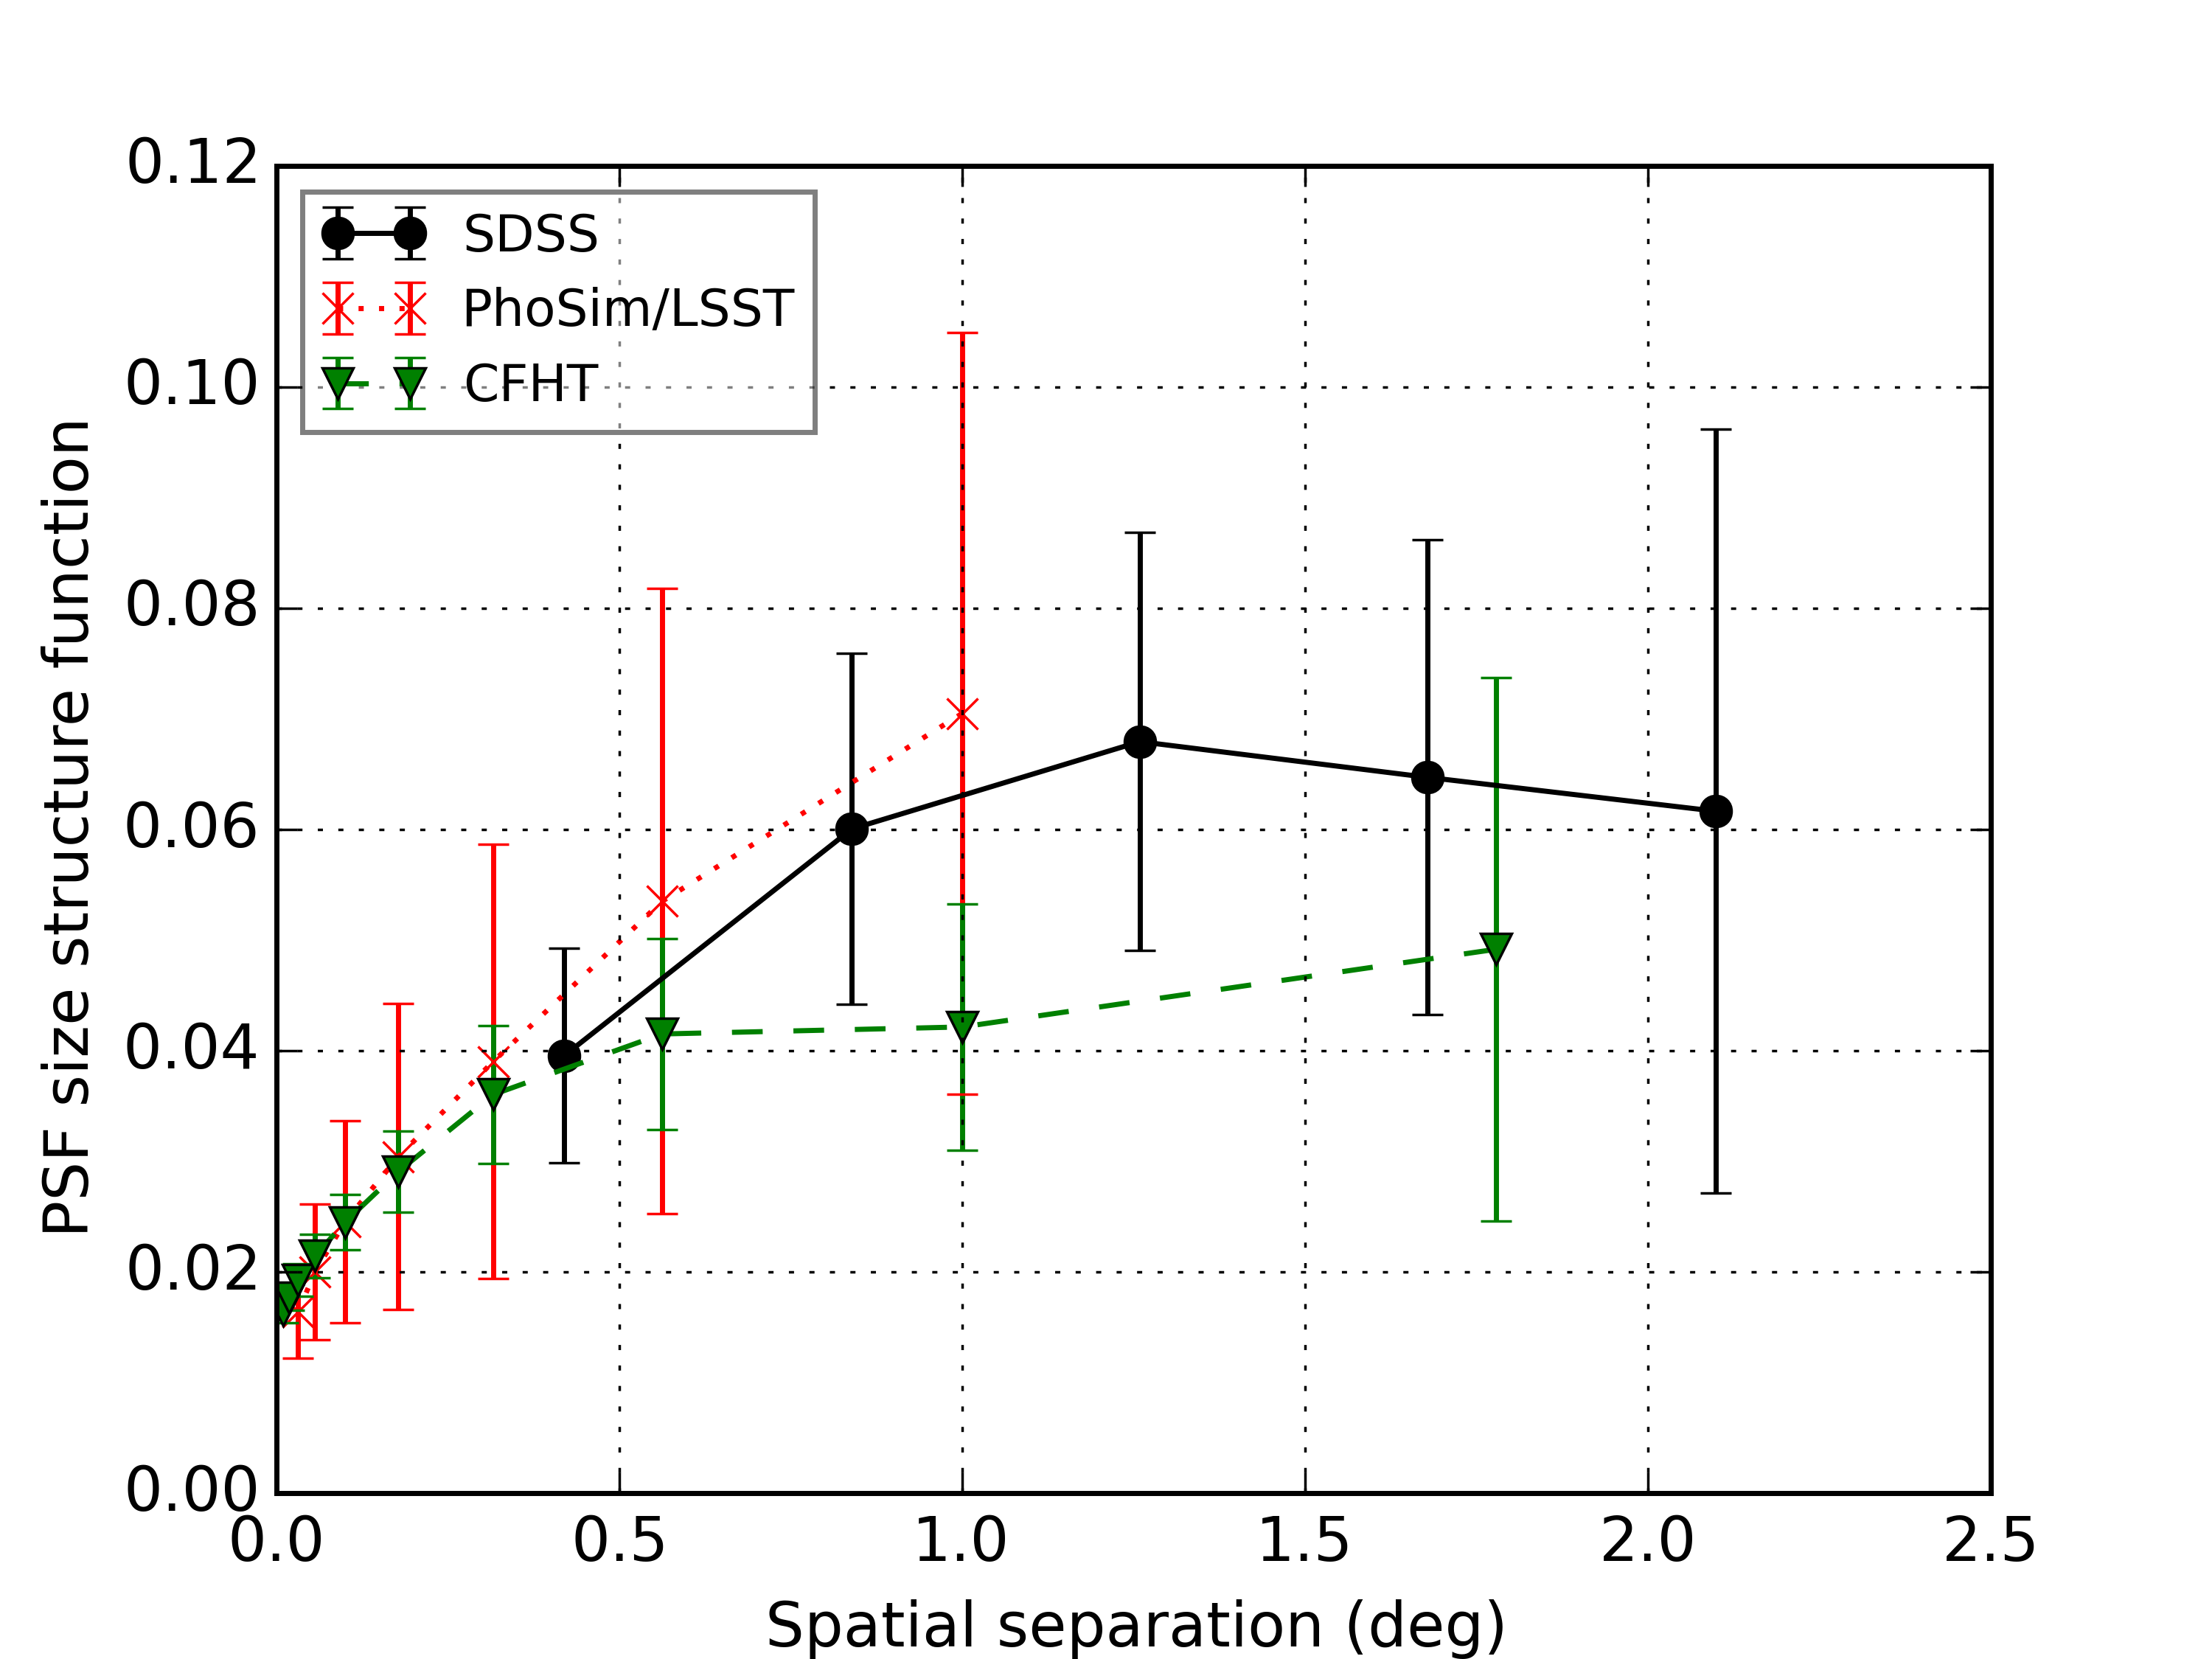
\includegraphics[width=0.8\textwidth]{FIGURES/spatial.png}
\caption{The angular structure function for the PSF size determined using 
  CFHT data from \cite{heymans2012}, SDSS data analyzed here, and LSST image simulations. 
  SDSS measurements are averaged over 86 runs with the number of fields larger than 100. 
\label{fig:spatial}}
\end{figure}

To examine the angular (spatial) correlation of the FWHM, we compute the angular
structure function using PSF measurements from all 6 camera columns.
Our structure function is defined as the root-mean-square scatter of the PSF size 
differences of pairs of stars in the same distance bin along the direction perpendicular
to the scanning direction\footnote{The adopted form 
of the structure function, $SF$, is closely related to the autocorrelation function, $ACF$, as 
$SF \propto (1-ACF)^{1/2}$.} .
The SDSS curves are combined for 86 Stripe 82 runs with the number of fields larger than 
100 (out of 108 runs) 
We also compared the structure functions for each band
separately, and found no statistically significant differences.
Results for the $r$-band are shown in Fig.~\ref{fig:spatial}.

The structure function starts saturating at separations of
$\sim 0.5 - 1.0$ degree, with an asymptotic value of about $\sim 0.05$ arcsec.
In other words, the seeing rms variation at large angular scales is about 5\%,
but we emphasize that our data do not probe scales beyond 2.5 degree. 

For comparison, Fig. ~\ref{fig:spatial} also shows results from the CFHT PSF 
measurements~\citep{heymans2012}, and simulated PSF angular
structure functions obtained using image simulation code PhoSim~\citep{phosim}. 
The PhoSim PSF profiles are obtained by simulating a grid of stars
spaced by 6 arcminutes with non-perturbed LSST telescope and ideal sensors.
The results are averaged over 9 different atmosphere realizations with
different wind and screen parameters and airmass, and over 3 different
wavelengths (350 nm, 660 nm, and 970 nm).
The CFHT PSF size measurements were made in the $i$-band, and provided
by the authors of~\cite{heymans2012}.
The three curves in Fig.~\ref{fig:spatial} appear to be quantitatively
consistent with each other, even though they correspond to telescopes at
different sites and with different optics. 

We note that the PhoSim code could be used to further quantitatively study the variation
of seeing with outer scale and the impact of telescope diameter; however,
such detailed modeling studies are beyond the scope of this report. 


\subsection{Temporal behavior}

\subsubsection{Power spectrum analysis} 

\begin{figure}[th]
\centering
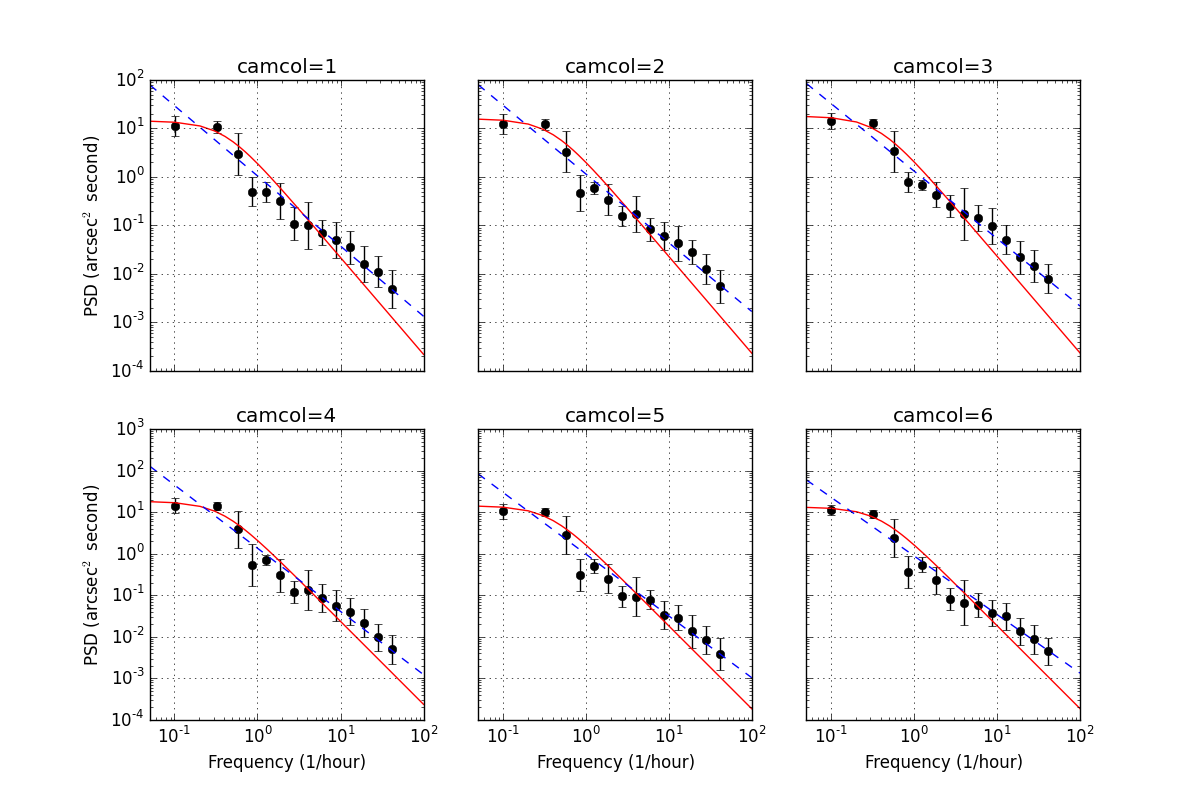
\includegraphics[width=0.99\textwidth]{FIGURES/temporalPSD.png}
\vskip -0.2in
\caption{PSF size temporal power spectral density for run 4874, r-band. 
The solid lines are fits using the damped random walk model. 
The dashed lines show best fits based on a single power law. The former
predicts a steeper high-frequency behavior, while the latter cannnot 
explain the turnover at low frequencies. 
\label{fig:psd}}
\end{figure}

To study the temporal behavior of the seeing, we first analyze its power spectrum.
Fig.~\ref{fig:psd} shows the temporal power spectral density (PSD) of the
PSF FWHM for 6 camera columns, in run 4874, $r$-band.
The time difference between subsequent fields is 36 seconds.
We fit the PSD using two competing models.
The first is a damped random walk (DRW) model~\citep[for introduction see Chapter 10 in][]{zeljkoBook},
\begin{equation}
\textrm{PSD}(f) = \frac{\tau^2 SF^2_{\infty}}{1+(2\pi f \tau)^2},
\end{equation}
where $f$ is the temporal frequency, $SF_{\infty}$ is the asymptotic
value of the structure function, and $\tau$ is the
characteristic timescale.
The solid curves in Fig.~\ref{fig:psd} show fits using this model.
Note that due to the lack of data toward the low-frequency end, the
first and second bins are four and two times wider than the
rest of the bins, respectively.
Combining fit results for all camera columns and optical bands for run 4874
gives $\tau = 23.6 \pm 1.3$ minutes.
Making the same fits for all the 108 runs in Stripe 82, 
we obtain the $\tau$ distribution vs. the duration of each
run, as shown in Fig.~\ref{fig:hist} (left).
The shorter runs tend to give smaller timescale. It is plausible that short runs 
cannot reliably constrain $\tau$ due to the lack of data toward the low-frequency 
end of the spectra. There are 12 runs longer than 6 hours and their characteristic timescales
are within the range of about $\sim5-30$ minutes.
This results is generally consistent with ~\cite{Racine1996}, where a timescale of 
$\tau = 17 \pm 1$ minutes was found.

The data consistently show a shallower high-frequency behavior than predicted
by damped random walk ($\propto 1/f^2$). In order to quantitatively describe 
the high-frequency tail of the PSD, we fit a simple power law,
\begin{equation}
\textrm{PSD}(f) = B f^\beta,
\end{equation}
where $B$ is the normalization factor, and $\beta$ is the power-law index.
Best-fits are illustrated for run 4874 are in Fig.~\ref{fig:psd} (dashed lines).
Combining fit results for all camera columns and filters gives $\beta = -1.29\pm 0.09$ 
for run 4874. Making the same fits for all the 108 runs in Stripe 82, we obtained the 
$\beta$ distribution vs. the duration of each run shown in Fig.~\ref{fig:hist} (right).
The shorter runs give $\beta$ values with a larger variance, but nevertheless it is 
clear that for most runs the high-frequency behavior can be described with a 
power-law index in the range $-1.5$ to $-1.0$. On the other hand, a single 
power law cannot explain the turnover at low frequencies. 

Therefore, neither model provides a satifactory fit over the entire frequency range: 
the power law fit systematically over predicts the low-frequency part of the PSD,
while the $1/f^2$ high-frequency behavior of damped random walk model is too 
steep. It is likely that a hybrid model would work, but we leave detailed analysis,
perhaps informed by the PhoSim modeling, for future work. 


\begin{figure}[th]
\centering
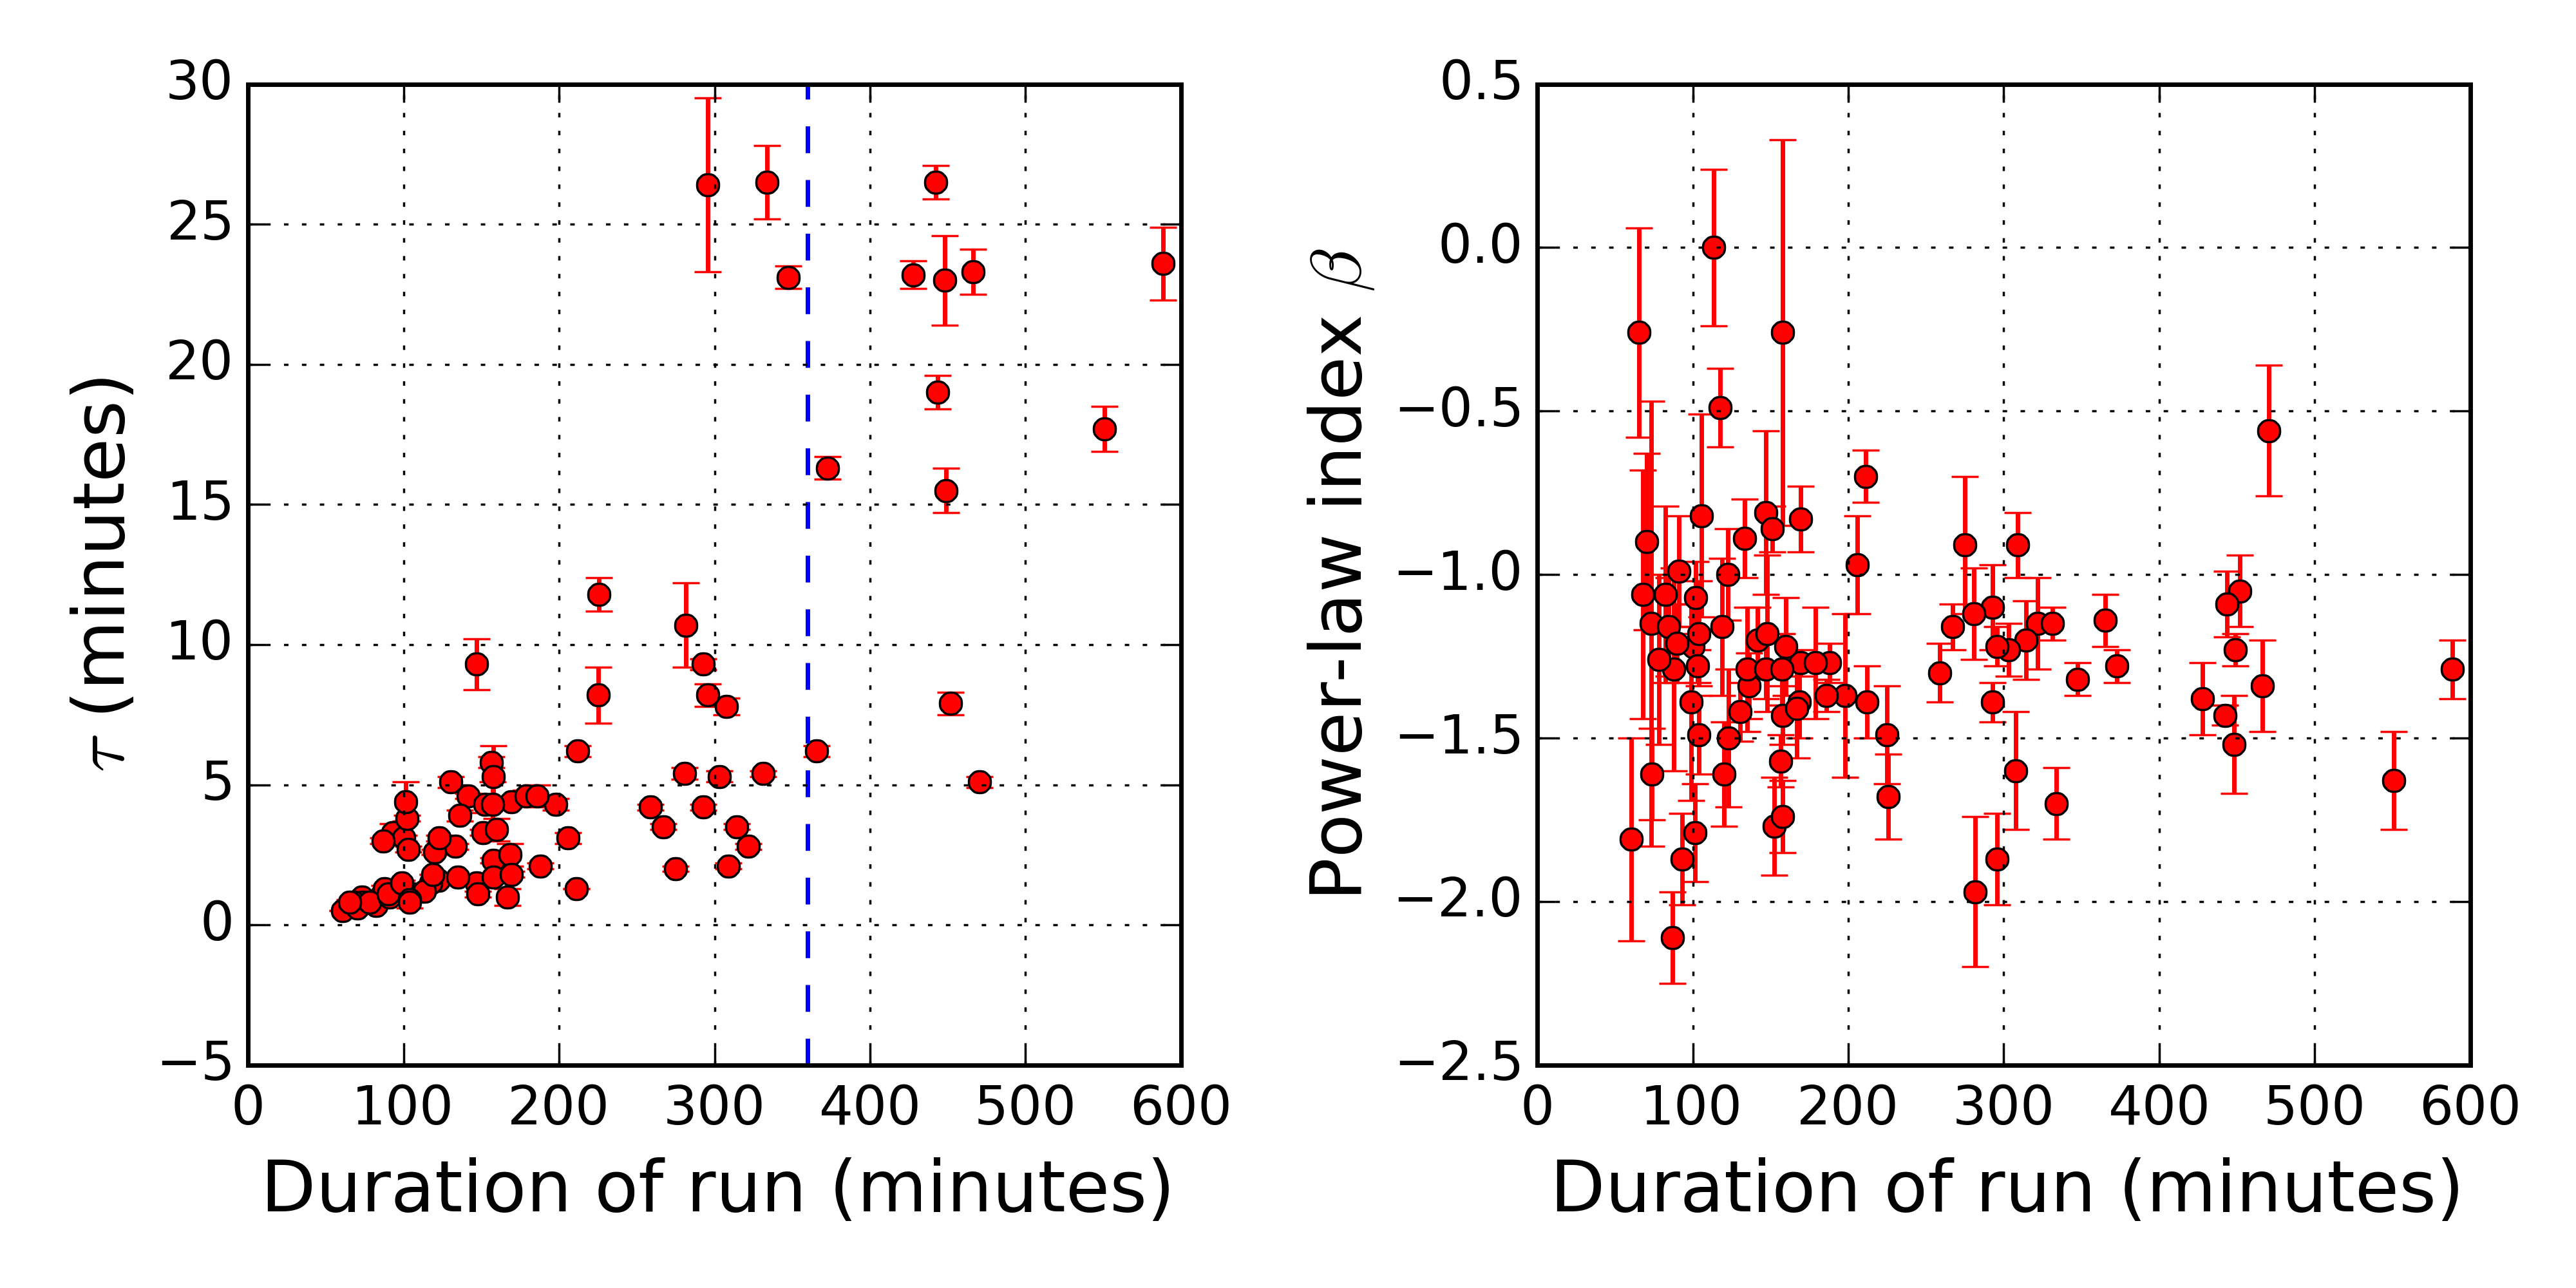
\includegraphics[width=0.99\textwidth]{FIGURES/taubeta.png}
\vskip -0.2in
\caption{Left: The symbols show the best-fit characteristic timescale $\tau$ in 
damped random walk for all 108 runs in Stripe 82 vs. the duration of 
each run. It is plausible that short runs cannot reliably constrain $\tau$.
Right: The power-law index $\beta$ for a single power law fit for all 108 
runs vs. the duration of each run. Note that for the majority of runs, $\beta$
is larger than the value appropriate for damped random walk ($\beta = -2$). 
\label{fig:hist}}
\end{figure}



\subsubsection{Structure function analysis} 


\begin{figure}[th]
\centering
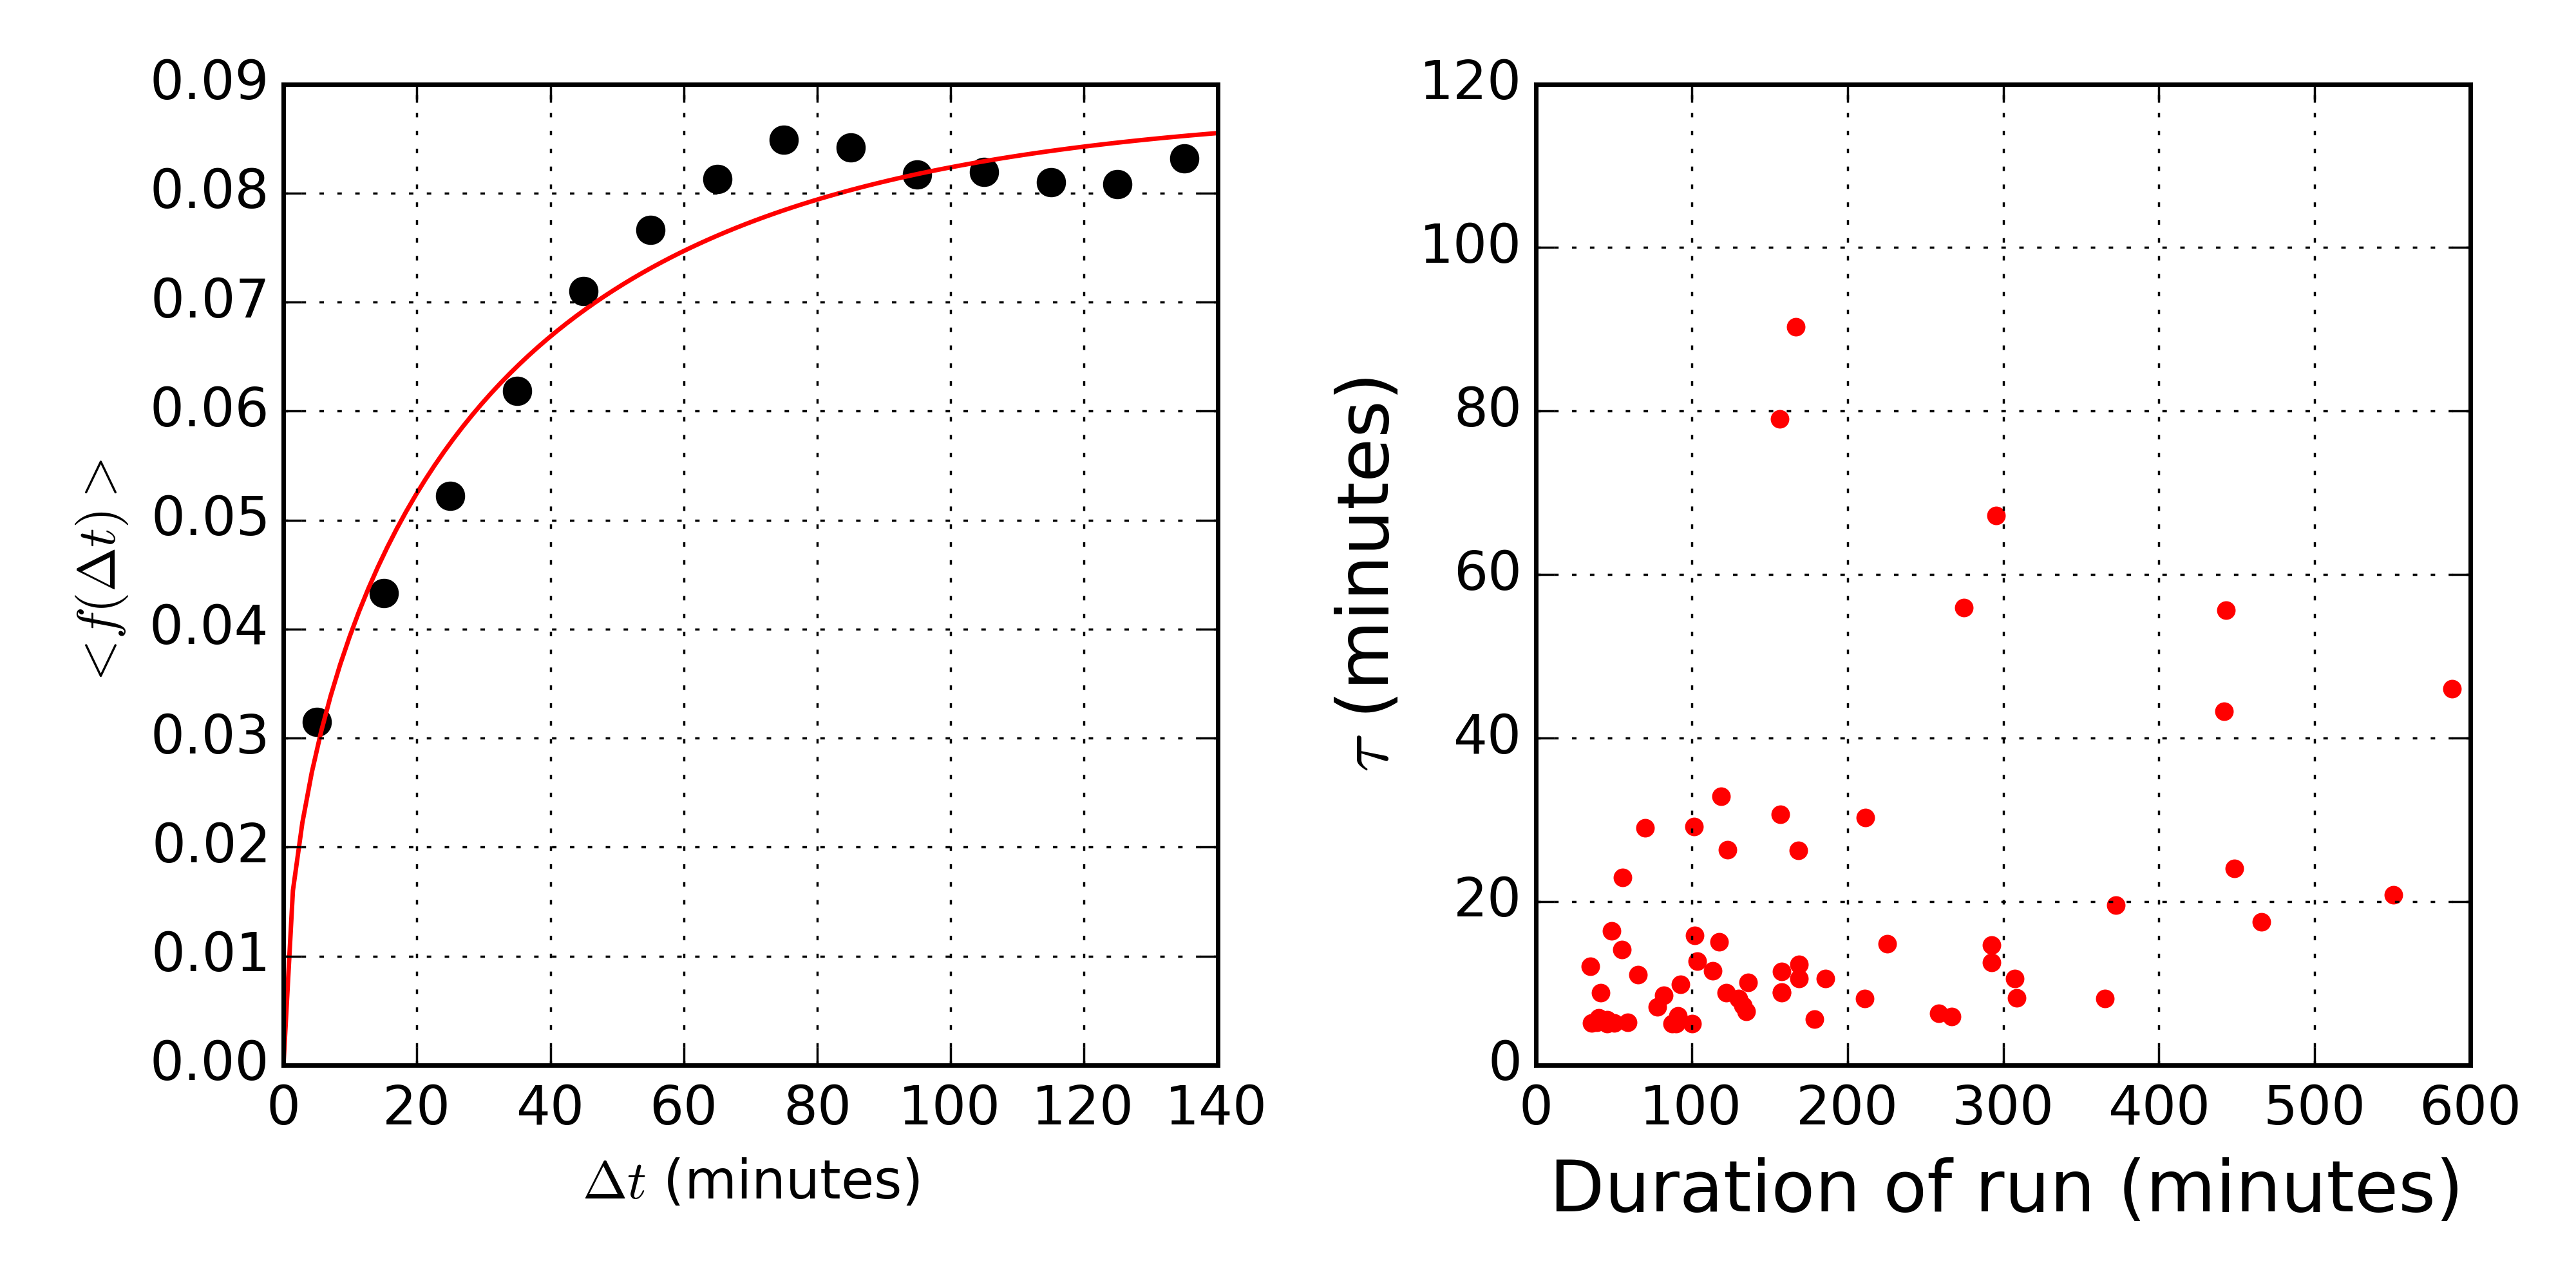
\includegraphics[width=0.9\textwidth]{FIGURES/fdt.png}
\caption{Left: The average normalized seeing difference, $<f(\Delta t)>$, as
  a function of the time separation, $\Delta t$, for run 4874, camera
   column 1, in the $r$-band. The fit to Eq.~(\ref{eq:fdt}) gives $f(\Delta t) ^\infty =  
   0.088\pm0.005$, $\tau = 45.1\pm10.3$ minutes and $\gamma$ =
   1.016$\pm$0.102. 
A damped random walk model has $\gamma=1$.
%The dashed line is the 
%   structure function predicted by damped random walk model with the same 
%   $f(\Delta t) ^\infty$ and $\tau$. 
Right: The timescale $\tau$ vs. the duration of each run.
 Note that for most runs $\tau$ is in the range 5-30 minutes
    ($\tau$ is set to zero for runs shorter than 20 minutes).  
\label{fig:fdt}}
\end{figure}


An alternative approach to power spectrum analysis is offered by auto-correlation 
and structure function analysis. Following~\cite{Racine1996}, we define a 
structure-function-like quantity
\begin{equation}
       f(\Delta t) = {| \theta(t+\Delta t) - \theta(t)| \over  \theta(t+\Delta t) + \theta(t) },
\end{equation} 
where $\theta$ is seeing. We then fit the mean value of $f(\Delta t)$ to 
\begin{equation}
    < f(\Delta t) > =  f(\Delta t) ^\infty \, \left( 1 - \exp[-(\Delta
      t/\tau)^\gamma] \right)^{1/2},
\label{eq:fdt}
\end{equation} 
with $f(\Delta t) ^\infty$, $\tau$ and $\gamma$ as free parameters.
Fig.~\ref{fig:fdt} (left) shows one example of such fits. This functional form is 
somewhat inspired by damped random walk model, where $\gamma=1$ and the 
term in brackets is raised to the power of a half. 
For this particular fit in Fig.~\ref{fig:fdt} (left), $\gamma$ is very close to 1.
%For illustration, Fig.~\ref{fig:fdt} 
%also shows a damped random walk model fit with the same $f(\Delta t) ^\infty$
%and $\tau$. 

The best-fit $\gamma$ is found to be mostly in the range 0.5 -1.5. 
The distribution of $\tau$ vs. 
the duration of each run is shown in Fig.~\ref{fig:fdt} (right) (somewhat 
arbitrarily, we set $\tau$ to zero for runs shorter than 20 minutes,
and those fits where the fitted $\tau$ is longer than 2/3 of the duration
of the run are deemed unreliable and not shown).  
%While the short runs show a larger variance in $\tau$, 
It is evident that 
for most runs the timescale $\tau$ is in the range 5-30 minutes.
Therefore, this analysis seems more robust at constraining the characteristic time
scale than fitting a damped random walk model to empirical PSD. 
